\documentclass[12pt, a4paper]{ctexart}
\usepackage{ctex}


\usepackage{graphicx}%图片包
\graphicspath{{figures/}}
%\includegraphics[scale=0.6]{.eps}\\

\usepackage{amsmath}%数学公式包
\usepackage{amssymb}%特殊符号包
\usepackage{bm}%加粗数学符号 \bm{math expression}
\usepackage{extarrows}%数学符号补充包 长等号

\usepackage{color}%Excel2LaTeX辅助包
\usepackage{booktabs}
\usepackage{multirow}
%\resizebox{120mm}{100mm}{} 调整表格大小
\usepackage{array}

\usepackage{listings}%插入代码
\lstset{language=Matlab}
\lstset{breaklines}%自动将长的代码行换行排版
\lstset{extendedchars=false}%解决代码跨页时,章节标题,页眉等汉字不显示的问题

\usepackage{geometry}
\geometry{left=1.5cm, right=1.5cm, top=2.5cm, bottom=2.5cm} %调整页边距
\usepackage{ulem}
\title{数理方程习题}
\author{中国语言文学系常代表办公室}
\renewcommand{\today}{\number\year /\number\month /\number\day}


\begin{document}
	\maketitle
	\iffalse
	%多行公式 &对齐
	\begin{align*}
	\\
	&=
	
	\end{align*}
	
	%圆括号矩阵
	$$A_1=
	\begin{pmatrix}
	&   &   &   &  \\
	&   &   &   &  \\
	%\dots \ddots \vdots
	\end{pmatrix}
	$$
	
	%靠左
	\begin{flushleft}
		\\
	\end{flushleft}
	
	%大括号表示
	$$x_{k+1} =
	\begin{cases}
	x_k+s_k & \text{if } \rho_k>\eta_1\\
	x_k & \text{otherwise} 
	\end{cases}$$
	
	%文字样式
	\uline{下划线}
	\uuline{双下划线}
	\uwave{波浪线}
	\sout{中间删除线}
	\xout{斜删除线}
	\dashuline{虚线}
	\dotuline{加点}
	\fi
	\newpage
	\tableofcontents
	\newpage
	\section{调和方程}
    \subsection{方程的物理背景和定解问题}
    \subsubsection{内容提要}
    
    \begin{itemize}
        \item 这门课研究什么?
        \begin{enumerate}
            \item 解方程 -- 但是方程大多数时候没有显式解
            \item 解的性质:适定性(存在性、唯一性、稳定性)
            \item 定解问题和定解条件:三类条件\quad Dirichlet, Neumann, Robin
        \end{enumerate}
        \item 调和函数(满足Laplace方程,齐次Possion方程): $-\Delta u = 0$,\\ Possion方程: $-\Delta u = f$.\\ 三类边值条件.\\ 外问题(通常需要给出$|x|\rightarrow\infty$时的边界条件,否则解可能不唯一).
        \item 变分原理:调和函数$\leftrightarrow$能量最(极)小元
        
        例:$$E(u) = \mathop{\inf}_{v\in U} E(v), \qquad E(v) := \int_{\Omega} \frac12 | \nabla v |^2 dx$$
        \item 背景知识
        \begin{enumerate}
            \item Green 公式(分部积分)
            微积分基本定理$$\int_a^bf'dx = f(b) - f(a)$$ \\
            分部积分公式$$\int_a^bf'gdx = fg\Big|_a^b - \int_a^bfg^{\prime}dx$$\\
            高维时(若$\Omega$光滑)
            $$ \begin{cases}
                \int_{\Omega} f_{x_i}dx = \int_{\partial \Omega}f \cdot \nu_i dS, \qquad\qquad \nu = (\nu_1, \dots, \nu_n) \text{为外法向} \\
                \int_{\Omega} f_{x_i}gdx = \int_{\partial \Omega}fg\nu_idS - \int_{\Omega}fg_{x_i}dx \\
                \end{cases}$$
            或者写成以下形式
            \begin{align*} 
            \int_{\Omega} \Delta f \cdot g dx &= - \int_{\Omega} \nabla f \cdot \nabla g dx + \int_{\partial \Omega} g \cdot \frac{\partial f}{\partial \bm{n}} dS \\
            &= \int_{\Omega} f \Delta g dx - \int_{\partial \Omega} f \frac{\partial g}{\partial\bm{n}}dS + \int_{\partial \Omega} g \frac{\partial f}{\partial\bm{n}}dS
            \end{align*}
            
            \item 常用引理:若$f \in C(\Omega)$且$\int_{\Omega} f \varphi dx \equiv 0, \forall \varphi \in C(\Omega)$,则$f\equiv0$.
            
            \item 常用公式: $ r = |y|, y \in \mathbb{R}^n $ 则$ \nabla r = \frac{y}{r}$,且$\Delta \frac1{|y|^{n-2}} = \Delta \frac1{r^{n-2}} = 0 (\forall n \geq 3)$,而$n=2$时有$\Delta \ln |r| = 0$.
            
            \item 场论中的常用符号及计算
            \begin{enumerate}
                \item 若$\bm f = P \bm i + Q \bm j + R \bm k $, 
                \begin{align*}
                \text{curl}\ \bm f &= \nabla \times \bm f = \left|
                \begin{array}{ccc}
                \bm i & \bm j & \bm k \\
                \partial_1 & \partial_2 & \partial_3 \\
                P & Q & R
                \end{array} \right| \\ 
                \text{div}\ \bm f &= \nabla \cdot \bm f = \partial_1  P + \partial_2  Q + \partial_3  R 
                \end{align*}
                \item div, curl都是线性的
                \item $ \nabla \cdot (f\bm a) = f \cdot (\nabla \cdot \bm a) + \nabla f \cdot \bm a$
                \item $ \nabla \times (f\bm a) = f \cdot(\nabla\times\bm a) + \nabla f \times \bm a$
                \item $ \nabla \cdot (\bm a \times \bm b) = \bm b (\nabla\times\bm a) - \bm a (\nabla\times\bm b)$
                \item $\nabla\times(\nabla f) = (\nabla \times \nabla) f = 0$\qquad 即:梯度无旋
                \item $\nabla \cdot (\nabla \times\bm a) = 0$ \qquad 即:旋度零散
                
            \end{enumerate}
            \item (习题$\S_{1.1}$第1-2题) Laplace算子在2维极坐标$(r, \theta)$,3维球坐标$(r, \theta, \varphi)$,3维柱坐标$(r, \theta, z)$下的表示:
            \begin{align*}
            \Delta u &= \frac1r \frac{\partial}{\partial r}(r\frac{\partial u}{\partial r}) + \frac1{r^2} \frac{\partial^2 u}{\partial \theta^2}\\
            \Delta u &= \frac1{r^2} \frac\partial{\partial r}(r^2\frac{\partial u}{\partial r}) + \frac1{r^2\sin\theta}\frac\partial{\partial \theta}(\sin\theta\frac{\partial u}{\partial\theta}) + \frac1{r^2\sin^2\theta}\frac{\partial^2u}{\partial\varphi^2}\\ 
            \Delta u &= \frac1r \frac\partial{\partial r}(r\frac{\partial u}{\partial r}) + \frac1{r^2}\frac{\partial^2u}{\partial\theta^2} + \frac{\partial^2u}{\partial z^2}
            \end{align*}
            
            \item (习题$\S_{1.1}$第5题)若$u(x)\in C^\infty$为$\mathbb{R}^n$上的调和函数,\\ 则$u(x)$在正交变换下保持调和.\\ {\bf Kelvin变换}:$$v(y) = \frac1{|y|^{n-2}}u\left(\frac{y}{|y|^2}\right),\qquad y\neq0,$$ $v$为$\mathbb{R}^n \backslash\{0\}$上的调和函数.
        
        \end{enumerate}
    
    \end{itemize}

    \subsubsection{$\S_{1.1}$第5(4)题}
    \kaishu{}
    若$u(x)\in C^\infty$为$\mathbb{R}^n$上的调和函数,\\ 则$u(x)$在正交变换下保持调和.\\ {\bf Kelvin变换}:$$v(y) = \frac1{|y|^{n-2}}u\left(\frac{y}{|y|^2}\right),\qquad y\neq0,$$ $v$为$\mathbb{R}^n \backslash\{0\}$上的调和函数.
    % todo: 检查证明
    
    \songti{}
    \uuline{解答}:\\
    最终要证明$\Delta v=0$,也就是要把$v_{yy}$通过$u_{yy}$通过$u_{xx}$表示出来,然后消掉得到0.
    
    首先,我们做一些准备工作,因为要用$u_{xx}$把$u_{yy}$表示出来,所以$x$会是中间变量,先做一些简单的整理,方便后续工作.记
    \begin{align*}
    x_i &= \frac{y_i}{|y|^2}\\
    \frac{\partial |y|^k}{\partial y_i} &= k \cdot y_i \cdot |y|^{k-2}\\
    \frac{\partial x_i}{\partial y_i} &= \frac{|y|^2-2y_iy_i}{|y|^4}\\
    \frac{\partial x_i}{\partial y_j} &= \frac{-2y_iy_j}{|y|^4},\qquad \forall i\neq j.\\
    \end{align*}
    利用复合函数求导性质$u=u(x), x(y) = \frac{y}{|y|^2}$,可以预见到的是接下来会出现$u_x,u_y,u_{xx},u_{yy},u_{xy}$.而$u_x$与$u_{xx}$最终要用于表示其它量,不用计算,直接保留,所以剩下3个量我们下面就开始算.
    \begin{align*}
    \frac{\partial u}{\partial y_i} &= \sum_j \frac{\partial u}{\partial x_j}\frac{\partial x_j}{\partial y_i} \\
    &= \frac{\partial u}{\partial x_i}\frac1{|y|^2} - 2\frac{y_i}{|y|^4}\sum_j\frac{\partial u}{\partial x_j}y_j;\\
    & \\
    \frac{\partial^2 u}{\partial y_j \partial x_i} &= \frac{\partial}{\partial x_i} (\frac{\partial u}{\partial y_j}) \\
    &= \frac{\partial^2 u}{\partial x_j \partial x_i}\frac1{|y|^2} - 2\frac{y_j}{|y|^4}\sum_k\frac{\partial^2 u}{\partial x_k \partial x_i} y_k;\\
    & \\
    \frac{\partial^2 u}{\partial y_i^2} &= \frac{\partial}{\partial y_i} (\frac{\partial u}{\partial y_i}) \\
    &= (\frac{\partial^2 u}{\partial y_i \partial x_i} \frac1{|y|^2} + \frac{\partial u}{\partial x_i}\frac{-2x_i}{|y|^2}) + (- \frac{\partial u}{\partial x_i}\frac{2x_i}{|y|^2} + \sum_j (\frac{\partial^2 u}{\partial y_i \partial x_j}\frac{2x_iy_j}{|y|^2} - \frac{\partial u}{\partial x_j}\frac{2y_j(|y|^2-4y_i^2)}{|y|^6})) \\
    &= \frac{\partial^2u}{\partial x_i^2}\frac1{|y|^4} + \frac{\partial u}{\partial x_i}\frac{(4-2n)x_i}{|y|^2}.
    \end{align*}
    算到这里,内心应该觉得平静.毕竟$u_{yy}$求和后确实能消掉2次项.接下来我们关注如何从$v_{yy}$算到$u_{yy}$.回忆一下,$v(y) = \frac1{|y|^{n-2}}u(\frac y{|y|^2})$,我们有
    \begin{align*}
    \frac{\partial v}{\partial y_i} &= \frac{\partial u}{\partial y_i}\frac1{|y|^{n-2}}+(2-n)u\cdot y_i \cdot \frac1{|y|^n};\\
    & \\
    \frac{\partial^2v}{\partial y_i^2} &= \frac{\partial}{\partial y_i}(\frac{\partial v}{\partial y_i}) \\
    &= (\frac{\partial^2u}{\partial y_i^2}\frac1{|y|^{n-2}} + \frac{\partial u}{\partial y_i}(2-n)\frac{y_i}{|y|^n}) + (\frac{\partial u}{\partial y_i}(2-n)\frac{y_i}{|y|^n} + (2-n)\cdot u \cdot (\frac1{|y|^n} - n\frac{y_i^2}{|y|{n+2}})).\\
    \end{align*}
    终于,我们可以算
    \begin{align*}
    \Delta v &= \sum_i \frac{\partial^2v}{\partial y_i^2} \\
    &= (\sum_i\frac{\partial^2u}{\partial y_i^2})|y|^{2-n} + (\sum_i \frac{\partial u}{\partial y_i}y_i)(4-2n)|y|^{-n}\\
    &= (\sum_i \frac{\partial^2u}{\partial x_i^2}\frac1{|y|^4} + \sum_i \frac{\partial u}{\partial x_i}\frac{(4-2n)x_i}{|y|^2})\cdot |y|^{2-n} + 
    (\sum_i(\frac{\partial u}{\partial x_i}\frac1{y^{2}} - \frac{2x_i}{|y|^2}\sum_j\frac{\partial u}{\partial x_j}y_j)\cdot y_i) \cdot(4-2n)\cdot |y|^{-n}\\
    &= \sum_i \frac{\partial u}{\partial x_i}\frac{(4-2n)x_i}{|y|^2} \cdot |y|^{2-n} + (\sum_i \frac{\partial u}{\partial x_i}\frac{-y_i}{|y|^2})\cdot(4-2n)\cdot|y|^{-n}\\
    &= 0.
    \end{align*}
    就证明了我们想要的结论.
    
    \subsubsection{$\S_{1.1}$第6题}
    \kaishu{}
    设$$J(u) = \frac12\int_{\Omega}| \nabla u |^2dx + \int_{\partial\Omega}(\frac12\sigma u^2-gu)dS,$$其中$\Omega$为n维区域.变分问题的提法为:求$u\in U$使得$$J(u) = \mathop{\inf}_{v\in U} J(v),$$其中$U=C^2(\Omega)\bigcap C^1(\bar{\Omega})$.试导出与此变分问题等价的边值问题,并证明两者的等价性.	
    
    % todo: 检查证明
    \songti{}
    \uuline{解答}:\\
    
    \uline{先证明变分问题可以推导出一个边值问题}:\\
    记 $f(t) = J(u+tw), w\in U$,则$f(t)$在$t=0$处取极小值,即
    \begin{align*}
    	0 = \left.\frac{df}{dt}\right|_{t=0} &=\left.\frac{d}{dt}\left(\frac12\int_{\Omega}| \nabla (u+tw) |^2dx + \int_{\partial\Omega}\left(\frac12\sigma (u+tw)^2-g(u+tw)\right)dS\right)\right|_{t=0}\\
    	&=\int_{\Omega}\nabla u \cdot \nabla w dx + \int_{\partial \Omega} (\sigma uw-gw)dS\\
    	&\xlongequal{\text{Green公式}}-\int_{\Omega} \Delta u \cdot w dx + \int_{\partial \Omega}\frac{\partial u }{\partial \bm{n}} w dS+\int_{\partial \Omega} (\sigma uw-gw)dS\\
    	&= -\int_{\Omega} \Delta u \cdot w dx + \int_{\partial \Omega} \left(\frac{\partial u }{\partial \bm{n}}  + \sigma u - g \right)wdS.
    \end{align*}
    考察满足$w|_{\partial\Omega} = 0 $的函数类,由背景知识第2条中的引理,易知 $ \Delta u = 0$,如此,方程变为
    $$ 0 = \int_{\partial \Omega}\left(\frac{\partial u }{\partial \bm{n}} + \sigma u - g\right)w dS = 0 \xLongrightarrow{\text{再由上述引理}} \frac{\partial u }{\partial \bm{n}} + \sigma u = g, \qquad \text{on}\ \partial \Omega.$$
    
    \uline{这个边值问题的解也是前述变分问题的解}:\\
    有\begin{align*}
    	J(u+w)& = J(u) + \frac12\int_{\Omega} |\nabla w|^2 dx+\frac12\int_{\partial \Omega} \sigma w^2 dx+ \int_{\Omega} \nabla u \cdot \nabla w dx + \int_{\partial \Omega}(\sigma u -g )w dS \\
    	&\xlongequal{\text{Green公式}}J(u)+ \frac12\int_{\Omega} |\nabla w|^2 dx+\frac12\int_{\partial \Omega} \sigma w^2 dx-\int_{\Omega} \Delta u \cdot w dx + \int_{\partial \Omega}\frac{\partial u }{\partial \bm{n}} w dS+ \int_{\partial \Omega}(\sigma u -g )w dS\\
    	&=J(u)+ \frac12\int_{\Omega} |\nabla w|^2 dx+\frac12\int_{\partial \Omega} \sigma w^2 dx-\int_{\Omega} \Delta u \cdot w dx + \int_{\partial \Omega} \left(\frac{\partial u }{\partial \bm{n}}  + \sigma u - g \right)wdS\\
    	&=J(u)+ \frac12\int_{\Omega} |\nabla w|^2 dx+\frac12\int_{\partial \Omega} \sigma w^2 dx\\
    	&\stackrel{\sigma>0}{\geq} J(u)
    \end{align*}

    \subsection{调和函数的基本性质及应用}
	\subsubsection{$\S_{1.2}$第9题}
	\kaishu{}
	设$u$为带状区域$\Sigma=\{(x_1,x_2)||x_1|\le 1, \quad -\infty<x_2< \infty\}$上的非负调和函数,证明:$$
	u(x)\le u(0)e^{C|x_2|},\quad \forall |x_1|\le \frac{1}{4},\quad -\infty<x_2< \infty		$$
	其中常数$C$不依赖于$u$.(提示:Harnack不等式)\\
	
	\songti{}
	\uuline{解答}:
	
	对于任意的$x=(x_1,x_2)\in \Sigma$,取半径为$\frac{3}{16}$的圆,用“滚圆法”折线连接$(x_1,x_2),(x_1,0),(0,0)$三点,假设总共需要N+2个圆$\{B_k\}_{k=1}^{N+2}$,那么第1,N,N+2个圆的圆心即为这三个点,记这些圆的圆心分别为$\{x^k\}_{k=1}^{N+2}$.
	
	
	此时满足注1.2.3的条件,可以使用Harnack不等式的推论,有
	\begin{align}
		u(x)&=u(x^1)\notag \\
		&\le C(n)u(x^2) \notag\\
		&\le (C(n))^2 u(x^3) \notag \\
		&\le \dots \notag \\
		&\le (C(n))^{N+1}u(x^{N+2}) \notag \\
		&= (C(n))^{N+1}u(0) \notag
	\end{align}\\
	且显然有
	\begin{align}
		&\qquad (N-1)\frac{3}{16} \le |x_2|	\notag \\
		&\Rightarrow N \le \frac{16}{3}|x_2| +1 \notag \\
		&\Rightarrow N+1 \le \frac{16}{3}|x_2| +2 \notag \\
		&\Rightarrow u(x) \le (C(n))^{\frac{16}{3}|x_2| +2}u(0) \notag 
	\end{align}\\
	{\color{red}{原题应当有误,右端还应该多一个常数.}}\\
	
	\subsubsection{$\S_{1.2}$第10题}
	\kaishu{}
	设$u \in C^2(\overline{\mathbb{R}_{+}^{n}})$为$\overline{\mathbb{R}_{+}^n}=\{(x_1,\dots,x_n)\in \mathbb{R}^n|x_n \ge 0\}$上的调和函数.若满足$u(x_1,\dots,x_{n-1},0)=0$且$u(x)$为有界函数,证明$u\equiv 0$.(提示:延拓为全空间调和函数)若把$u$改为下有界函数,试举出例子使得结论不成立.\\
	
	\songti{}
	\uuline{解答}:
	
	对$x=(x_1,x_2,\dots,x_n)\in \mathbb{R}^n$,定义$\bar{x}=(x_1,x_2,\dots,-x_n)$.	

	我们给出$u$的全空间调和延拓的构造,然后应用Liouville型定理即可.$$
	v(x)=\begin{cases}
	u(x) & \text{if } x_n \ge 0\\
	\overline{u(\bar{x})} & \text{if } x_n < 0
	\end{cases}$$
	若把$u$改为下有界函数,结论不成立,反例有$u(x)=x_n$.
	
	\subsubsection{$\S_{1.2}$第11题}
	\kaishu{}
	若$u$为$\mathbb{R}^2$上的调和函数.设$0<a\le b\le c$满足$b^2=ac$,证明$$
	\int_{\mathbb{S}^1} u(x^0+a\omega)u(x^0+c\omega)dS_{\omega}=\int_{\mathbb{S}^1}
	u^2 (x^0+b\omega)dS_{\omega}	$$
	(提示:固定$b$后,对上式左端求导.)上述结论对一般维数$\mathbb{R}^n$也成立,有兴趣的同学可以自己证明.\\
	
	\songti{}
	\uuline{解答}:
	
	固定b,记$f(a)=\int_{\mathbb{S}^1} u(x^0+a\omega)u(x^0+\frac{b^2}{a}\omega)dS_{\omega}$,只要证明$f^{'}(a)=0$即可.
	\begin{align*}
		&\qquad f^{'}(a)=\int_{\mathbb{S}^1}\omega\cdot \nabla u(x^0+a\omega)u(x^0+\frac{b^2}{a}\omega)dS_{\omega} -\frac{b^2}{a^2}\int_{\mathbb{S}^1}\omega\cdot \nabla u(x^0+\frac{b^2}{a}\omega) u(x^0+a\omega)dS_{\omega} \\
		&=\frac{1}{a} \left(\int_{\mathbb{S}^1}a\omega\cdot \nabla u(x^0+a\omega)u(x^0+\frac{b^2}{a}\omega)dS_{\omega} -\int_{\mathbb{S}^1}\frac{b^2}{a}\omega\cdot \nabla u(x^0+\frac{b^2}{a}\omega) u(x^0+a\omega)dS_{\omega}\right)	\\
		&=\frac{1}{a} \left(\int_{\mathbb{S}^1}\frac{\partial u(x^0+aw)}{\partial n_{\omega}}u(x^0+\frac{b^2}{a}\omega)dS_{\omega} -\int_{\mathbb{S}^1}\frac{\partial u(x^0+\frac{b^2}{a}w)}{\partial n_{\omega}} u(x^0+a\omega)dS_{\omega}\right)	\\
		&\stackrel{\text{Green第二公式}}{=}\frac{1}{a} \left(\iint_{B_1}\Delta u(x^0+aw)u(x^0+\frac{b^2}{a}\omega)d\omega -\iint_{B_1} \Delta u(x^0+\frac{b^2}{a}w) u(x^0+a\omega)d\omega\right)	\\
		&=0 \notag
	\end{align*}
	
    \subsection{极值原理及其应用}
	\subsubsection{$\S_{1.3}$第2题}
	\kaishu{}
	对一般的椭圆型方程$$
	\sum_{i,j=1}^{n}a_{ij}\frac{\partial^2 u}{\partial x_i \partial x_j}+\sum_{i=1}^{n}b_i \frac{\partial u}{\partial x_i}+cu=0$$
	其中$(a_{ij})$为正定阵,$c\le 0$.证明弱极值原理,强极值原理成立.\\
	
	\songti{}\uuline{解答}:
	
	首先我们必须叙述清楚一般椭圆型方程极值原理的含义.\\
	
	\uwave{弱极值原理}:
	
	若$u\in C^2(B_1) \cap C(\bar{B_1})$,满足一般椭圆方程,则$u$不能在$B_1$内部取到非负最大值/非正最小值.
	
	\uwave{强极值原理}:
	
	若$u\in C^2(B_1) \cap C(\bar{B_1})$,满足一般椭圆方程.设$x^0\in \partial B_1$,使得$$
	u(x^0)>u(x),\forall x \in B_1$$
	则有$$
	\liminf_{t \to 0^+} \frac{u(x^0)-u(x^0-t\bm{n})}{t} >0 $$
	其中$\bm{n}$为$\partial B_1$在$x_0$处的单位外法向量.\\
	
	证明:
	
	先证弱极值原理.记题中方程左端为$L(u)$,其中$L$是椭圆型微分算子,容易验证它是线性的.则椭圆型方程可以简写成$L(u)=0$.只证明非负最大值不能在内部取得.我们先考虑$L(u)>0$时的情形,然后用摄动的方法推证$L(u)=0$时也成立.
	
	$L(u)>0$,用反证法,假设$\exists x_0 \in B_1$,使得$u$在$x_0$处达到了非负最大值.那么有
	$$
	\begin{cases}
	\left.u\right|_{x_0} &\ge 0  \\
	\left. \frac{\partial u}{\partial x_i}\right|_{x_0} &=0 , \forall i  \\ \left.H=\left( \frac{\partial^2 u}{\partial x_i \partial x_j}\right)_{i,j} \right|_{x_0}&\le 0  
	\end{cases}$$
	但是,在${x_0}$处,有$$
	\sum_{i,j=1}^{n}a_{ij}\frac{\partial^2 u}{\partial x_i \partial x_j}>-cu\ge 0
	$$
	记$A=(a_{ij})$,则它是正定阵,那么在${x_0}$处,有
	\begin{align}
	&\qquad \sum_{i,j=1}^{n}a_{ij}\frac{\partial^2 u}{\partial x_i \partial x_j}> 0\notag\\
	&\Rightarrow tr(AH)>0\notag \\
	&\Rightarrow tr(C^T CH)>0 ,\exists C \in \mathbb{R}^{n \times n}\notag \\
	&\Rightarrow tr(CHC^T)>0 \notag\\
	&\Rightarrow \text{H正定,矛盾!}\notag 
	\end{align}
	
	下面考虑一般的情形,取$h=e^{kx_1}$,其中$k>0$,考察函数$u_{\epsilon}=u+\epsilon h$,有$L(u_{\epsilon})=L(u+\epsilon h)=L(u)+\epsilon L(h)=0+\epsilon(a_{11}k^2+b_1 kh+ch)h$,我们希望有$L(u+\epsilon h)>0$,可以取$h$足够大,那么对足够小的$\epsilon$,$u_{\epsilon}$的非负最大值恒在边界上取得,考虑到$u_{\epsilon}$的连续性,令$\epsilon \to 0$,即得证.
	
	下面证明强极值原理.我们希望构造函数$w=u-v$,对$w$使用弱极值原理.而函数$v$满足
	$$\begin{cases}
	\left.v\right|_{\partial B_1} =0\\
	L(v)<0,in \quad B_1\backslash B_{\frac{1}{2}} \\ 
	\frac{\partial v}{\partial \bm{n}}>0
	\end{cases}$$
	可以取$$
	v=v_\alpha=e^{-\alpha}-e^{-\alpha r^2}$$
	取$\alpha$足够大就可以满足上面的要求,剩下的工作和书上的做法是类似的.\\
	
	{\color{red}{在新版教材上,删去了常数$c$,那么极值原理的描述就与书上的一样了.}}
	
	\subsubsection{$\S_{1.3}$第4题}
	\kaishu{}给出一个函数$\varphi$的例子,满足定理1.3.3中截断函数的性质.\\
	
	\songti{}\uuline{解答}:
	%可以用C无穷的函数作变限积分的上下限——王旭磊
	首先我们给出所需要的性质:$$
	\varphi(x)=\begin{cases}
	1 &  x\in B_{\frac{1}{2}}\\
	0 &  x \in B_1 \backslash B_{\frac{3}{4}}
	\end{cases}	\qquad \varphi \in C_{c}^{\infty}(B_1)$$
	
	考虑使用磨光算子的方法.
	
	考察$$
	\bar{\varphi}(x)=	\begin{cases}
	\frac{1}{e^{|x|^2-1}} & \text{if } |x|<1\\
	0 & \text{if }  |x| \ge 1
	\end{cases}$$ \\
	显然,$\bar{\varphi} \in C_{c}^{\infty}(\mathbb{R}^n),supp(\bar{\varphi})=B_1$,我们记$$
	c=\int_{\mathbb{R}^n} \bar{\varphi}(x)dx	$$\\
	如果$$
	\alpha(x)=\frac{1}{c}\bar{\varphi}(x)	$$\\
	那么$$
	\int_{\mathbb{R}^n} \alpha(x)dx=1	$$\\
	下面构造一簇$\epsilon$-相关的函数$$
	\alpha_{\epsilon}(x)=\frac{1}{\epsilon^n}\alpha\left(\frac{x}{\epsilon}\right)	$$\\
	则$\alpha_{\epsilon} \in C_{c}^{\infty}(\mathbb{R}^n),supp(\alpha_{\epsilon})=B_{\epsilon},\text{并且}\int_{\mathbb{R}^n} \alpha_{\epsilon}(x)dx=1$.直观上,$\alpha_{\epsilon}$这个函数的主要部分都集中在一个很小的球内.
	
	我们只在径向上考虑这个问题,取$$
	\psi(x)=	\begin{cases}
	1 & \text{if } |x|\le \frac{5}{8}\\
	0 & \text{if }  |x| > \frac{5}{8}
	\end{cases}$$ \\
	令
	\begin{align}
		\varphi(x)&=\psi(x)\ast \alpha_{\epsilon} \notag \\
		&= \int_{\mathbb{R}^n} \psi(y) \alpha_{\epsilon}(x-y) dy  \notag
	\end{align}
	可以看到,积分区域其实是$\{ \left. y\right| |x-y| \le \epsilon \} $,因此我们可以取$\epsilon=\frac{1}{16}$.由卷积转移求导的性质,易见径向函数$\varphi(x)$即为所求.
	
	\subsubsection{$\S_{1.3}$第6题}
	\kaishu{}证明球$B_R$上的梯度估计:若$u \in C^2(B_R) \cap C(\bar{B}_R)$为调和函数,则成立$$
	\sup_{B_{\frac{R}{2}}} |\nabla u| \le \frac{c(n)}{R} \sup_{\partial B_R}|u|,	$$
	其中$c(n)$为只依赖于空间维数$n$的正常数.\\
	
	\songti{}\uuline{解答}:\\
	
	两种做法,其一是使用Bochner技巧,依照书上的推导过程再写一遍,只要将$R$固定,取新的截断函数$\varphi_R(x)=\varphi\left(\frac{x}{R} \right)$即可.
	
	另一种做法是直接利用单位球$B_1$上的梯度估计.
	
	对于上述的函数$u$,构造函数$v(x)=u(Rx)$,于是$v \in C^2(B_1) \cap C(\bar{B}_1)$,所以
	\begin{align}
	&\qquad \sup_{B_{\frac{1}{2}}} |\nabla v| \le c(n) \sup_{\partial B_1}|v| \notag \\
	&\Rightarrow R \sup_{B_{\frac{R}{2}}} |\nabla u| \le c(n) \sup_{\partial B_R}|u| \notag \\
	&\Rightarrow \sup_{B_{\frac{R}{2}}} |\nabla u| \le \frac{c(n)}{R} \sup_{\partial B_R}|u| \notag.
	\end{align}	\\
    
	\subsubsection{$\S_{1.3}$第7题}
	\kaishu{}利用梯度估计证明若$u \in C^{\infty}$为$\mathbb{R}^n$上的调和函数, 且存在自然数$k$ 使得$$
	|u(x)| \sim |x|^k,\quad x \to \infty.$$
	则$u $必为$k $阶多项式.(这些多项式称为调和多项式.)\\
	
	\songti{}\uuline{解答}:\\
	
	所谓存在自然数$k$ 使得$|u(x)| \sim |x|^k,\quad x \to \infty$,即$\exists c_1,c_2 >0, c_1|x|^k \le u(x) \le c_2|x|^k , x\to \infty.$事实上,如果承认调和函数的解析性,这个问题就变得十分容易,但这里一定要用梯度估计来做.我们分两步证明这个问题.
	\begin{enumerate}
		\item  $u(x)$是不超过$k$次的多项式;
		\item  $u(x)$的增长阶不低于$k$次多项式.
	\end{enumerate}
	事实上,第二步由$|u(x)| \sim |x|^k,\quad x \to \infty$马上就可以得到,我们只证明第一步.\\
	由梯度估计\begin{align*}
		\sup_{B_{\frac{R}{2}}} |\nabla u| &\le \frac{c(n)}{R} \sup_{\partial B_R}|u|\\
		&\stackrel{R\text{足够大}}{\le} \frac{c(n)}{R} c_2|R|^k\\
		&\xlongequal{c(n)\cdot c_2\text{仍记作}c(n)} c(n)R^{k-1}\\
		&=c(n)\left(\frac{R}{2}\right)^{k-1} \cdot 2^{k-1}\\
		&\xlongequal{c(n)\cdot 2^{k-1}\text{仍记作}c(n)}c(n)\left(\frac{R}{2}\right)^{k-1}.
	\end{align*}
	即$R$足够大时,有$$
	\sup_{B_R} |\nabla u| \le c(n) R^{k-1}.$$
	由于$u\in C^{\infty}$(事实上这是个多余的条件),$\nabla u$的每一个分量都是调和函数.且$\forall i,\sup_{B_R} |\partial_i u| \le c(n) R^{k-1}. $如此,重复上面的过程,我们可以得到$$
	\sup_{B_R} |\nabla (\partial_i u)| \le c(n) R^{k-2}.	$$
	有限维情形下,总是$$\exists c>0,\quad \sup_{B_R}|\nabla^2 u| \le c\sup_{B_R} \sum_{i=1}^n|\nabla (\partial_i u)|\le c(n) R^{k-2}. $$
	迭代有限次,便可以得到$$
	\sup_{B_R} |\nabla^{k+1} u| \le c(n) R^{-1}.$$
	在上面令$R \to \infty$,得到$\sup_{\mathbb{R}^n} |\nabla^{k+1} u|=0.$做有限次积分就可以得到要证的结论.
	
    \subsection{格林函数法}
    	
    \subsubsection{$\S_{1.4}$第2题}
    \kaishu{}证明Green函数的性质1-4.\\
    \begin{enumerate}
    	\item $G(x,y)=0,x \in \Omega,y \in \partial \Omega,
    	$\item $G(x,y) \in C^2(\bar{\Omega}\times \bar{\Omega} \backslash \{y=x\}),$满足$$
    	0\le G(x,y) \le \begin{cases}
    	\Gamma(x-y), &n \ge 3\\
    	\Gamma(x-y)+\frac{1}{2\pi}lndiam(\Omega), &n=2.
    	\end{cases}	$$
    	当$y \to x$时,$G(x,y) \to + \infty$,其阶数和$\Gamma(x-y)$相同.
    	\item $G(x,y)=G(y,x), \qquad \forall x,y \in \Omega, y \ne x.
    	$\item $\int_{\partial \Omega} \frac{\partial G(x,y)}{\partial \bm{n}_x}dS_x =-1, \qquad \forall y \in \bar{\Omega}.$
    \end{enumerate}
    
    
    \songti{}\uuline{解答}:\\
   
    \begin{enumerate}
    	\item  由定义这是显然的,另外由性质3还可以得到$G(x,y)=0,x \in  \partial \Omega,y \in\Omega.$
    	\item 由定义,$\gamma(x,y)$在$\Omega$上调和,且在边界上取有限值,于是$|\gamma(x,y)|$在$\bar{\Omega}$上有上界$M < \infty$.又$\Gamma(x-y)$在$\{y=x\}$附近趋于$+\infty$,因此$\exists r >0, s.t. \left.\Gamma(x-y)\right|_{y\in  B_r(x)\backslash \{x\}}>M.$如此定义$\Omega_r=\bar{\Omega}\backslash B_r(x)$,易见$G(x,y)=\Gamma(x-y)-\gamma(x-y)$在$\Omega_r$上调和,且在$\partial \Omega_r$上取值恒非负,由调和函数的极值原理,可以得到$$
    	G(x,y)\ge 0 , \qquad \forall y \in \Omega_r	$$
    	再结合$\Omega_r$满足的条件,可以得到左边的不等号成立.\\
    	另外一边,由定义,$\gamma(x,y)$在$\Omega$上调和,于是由极值原理$$
    	\max_{y\in \bar{\Omega}}\gamma(x,y)=\max_{y\in \partial\Omega}\gamma(x,y)=\max_{y\in \partial\Omega}\Gamma(x-y).	$$
    	同样\begin{align*}
    	\min_{y\in \bar{\Omega}}\gamma(x,y)
    	&=\min_{y\in \partial\Omega}\gamma(x,y)\\
    	&=\min_{y\in \partial\Omega}\Gamma(x-y)\\
    	&=\begin{cases}
    	\min_{y\in \partial\Omega} \frac{1}{(n-2)w_{n-1}}\frac{1}{|x-y|^{n-2}} & n\ge 3\\
    	\min_{y\in \partial\Omega} \frac{1}{2\pi}ln \frac{1}{|x-y|} & n=2
    	\end{cases}\\
    	&\ge \begin{cases}
    	0 &n \ge 3\\
    	-\frac{1}{2\pi}ln diam\Omega &n=2.
    	\end{cases}
    	\end{align*}
    	于是$$
    	G(x,y)=\Gamma(x-y)-\gamma(x-y) \le \begin{cases}
    	\Gamma(x-y) &n \ge 3\\
    	\Gamma(x-y)+\frac{1}{2\pi}ln diam\Omega &n=2.
    	\end{cases}	$$
    	最后$$
    	\lim_{y \to x} \left|\frac{G(x,y)}{\Gamma(x-y)} \right|=\lim_{y \to x} \left| 1-\frac{\gamma(x,y)}{\Gamma(x-y)}\right| \xlongequal{\gamma\text{调和}}0.	$$
    	\item 只要证明$\left.G(x,z)\right|_{z=y} = \left.G(y,z)\right|_{z=x}.$而$$
    	G(x,z)\in C^2(\Omega \backslash \overline{Br(x)}) \cap C^1(\overline{\Omega \backslash Br(x)})	$$ $$
    	G(y,z)\in C^2(\Omega \backslash \overline{Br(y)}) \cap C^1(\overline{\Omega \backslash Br(y)})$$
    	这两个函数的定义域严格而言并非完全相同,但几乎是差不多的,因此我们考虑这样的区域:$$
    	\tilde{\Omega}:=\Omega \backslash (\overline{B_{\epsilon}(x)} \cup \overline{B_{\epsilon}(y)})	.$$
    	其中,$\epsilon$满足$\overline{B_{\epsilon}(x)} \cap \overline{B_{\epsilon}(y)} =\varnothing. $为了简化书写,我们记$$
    	v(z):=G(x,z),\qquad w(z):=G(y,z),	$$
    	在$\tilde{\Omega}$上,我们可以使用Green公式
    	\begin{align*}
    	&\qquad \int_{\tilde{\Omega}}(w \Delta v- v \Delta w)dx =\int_{\partial \tilde{\Omega}}\left( w\frac{\partial v}{\partial \bm{n}}-v\frac{\partial w}{\partial \bm{n}} \right)dS_z\\
    	&\xLongrightarrow{v,w \text{的基本性质}}\int_{\partial B_{\epsilon}(x)}\left( w\frac{\partial v}{\partial \bm{n}}-v\frac{\partial w}{\partial \bm{n}} \right)dS_z=\int_{\partial B_{\epsilon}(y)}\left( w\frac{\partial v}{\partial \bm{n}}-v\frac{\partial w}{\partial \bm{n}} \right)dS_z.
    	\end{align*}
    	再由与Green恒等式的推导类似的过程,令$\epsilon \to 0$,便可以得到$w(x)=v(y)$,这就是我们要证的.
    	\item 在表达式$$
    	u(x)=-\int_{\Omega}G(x,y)\Delta u(y)dy-\int_{\partial \Omega}u(y)\frac{\partial G}{\partial \bm{n}_y}(x,y)dS_y	$$
    	中,取$u(x) \equiv 1$即可.
    \end{enumerate}

	\subsubsection{$\S_{1.4}$第3题}
	\kaishu{}验证2维圆盘的Green函数和半空间的Green函数公式成立.\\
	
	\songti{}\uuline{解答}:
	
	考虑$x\in B_R$关于$\partial B_R$的反演点$$\tilde{x}=\frac{R^2 }{|x|^2}x.$$
	电势函数为$$
	\Gamma (x-y)=\frac{1}{2\pi}	ln\frac{1}{|x-y|}.$$
	限制在边界$y\in \partial B_R$上时,我们有
	\begin{align}
		\Gamma(\tilde{x}-y)&=\frac{1}{2\pi}	ln\frac{1}{|\tilde{x}-y|} \notag\\
		&=\frac{1}{2\pi} ln\frac{1}{|\frac{R^2 }{|x|^2}x-y|} \notag \\
		&=\frac{1}{2\pi} \left( ln\frac{|x|}{R}+ln \frac{1}{|x-y|} \right) \notag \\
		&=\frac{1}{2\pi} ln\frac{|x|}{R}+ \Gamma (x-y) \notag .
	\end{align}
	则令
	\begin{align}
		\gamma(x,y) &= \Gamma(\tilde{x}-y)-\frac{1}{2\pi} ln\frac{|x|}{R} \notag\\
		&= \frac{1}{2\pi} ln\left( \frac{R}{|x|} \cdot\frac{1}{|\tilde{x}-y|} \right)\notag.
	\end{align}
	如此,Green函数
	\begin{align}
		G(x,y)&=\Gamma(x-y) -\gamma(x,y)\notag\\
		&=\frac{1}{2\pi} ln\frac{1}{|x-y|}-\frac{1}{2\pi} ln\left( \frac{R}{|x|} \cdot\frac{1}{|\tilde{x}-y|}\right) \notag\\
		&= \frac{1}{2\pi} ln\frac{1}{|x-y|}- \frac{1}{2\pi} ln \left| \frac{R}{|x|}x-\frac{|x|}{R}y\right| \notag
	\end{align}
	便完成了构造.至于上半平面的Green函数,构造起来非常容易,问题在于验证衰减性条件可以保证Green恒等式仍然成立.我们将这个问题作为一个独立的题目,在下一个习题中给出解答.
	
	\subsubsection{$\S_{1.4}$第6题}
	\kaishu{}证明$u$满足(1.59)时,Green恒等式(1.47)依然成立.\\
	
	\songti{}\uuline{解答}:\\
	
	(1.59)即:$$
	u(x)=o(1),\qquad |\nabla u(x)|=o\left( \frac{1}{|x|} \right), \qquad |x| \to \infty.	$$
	要证的Green恒等式(1.47)为$$
	u(x)= -\int_{\Omega} \Gamma(x-y) \Delta u(y) dy + \int_{\partial \Omega} \left(\Gamma(x-y) \frac{\partial u}{\partial \bm{n}_y}(y) -u(y)\frac{\partial \Gamma}{\partial \bm{n}_y}(x,y)   \right) dS_y.	$$
	
	%有人认为条件(1.59)只是针对$n \ge 3$而言的,若$n=2$,应有更强的衰减条件,这里面可能有一个mistake.
	
	此时$\Omega$是无界区域,我们希望使用有界区域去逼近之.记$\Omega_R=\Omega \cap B_R(x) ,\quad \gamma_1= \partial\Omega_R \backslash \partial B_R(x) ,\quad \gamma_2= \partial\Omega_R \backslash \partial \Omega $,如图\ref{pde1_4_6}所示.
	\begin{figure}[htbp]
		\centering
		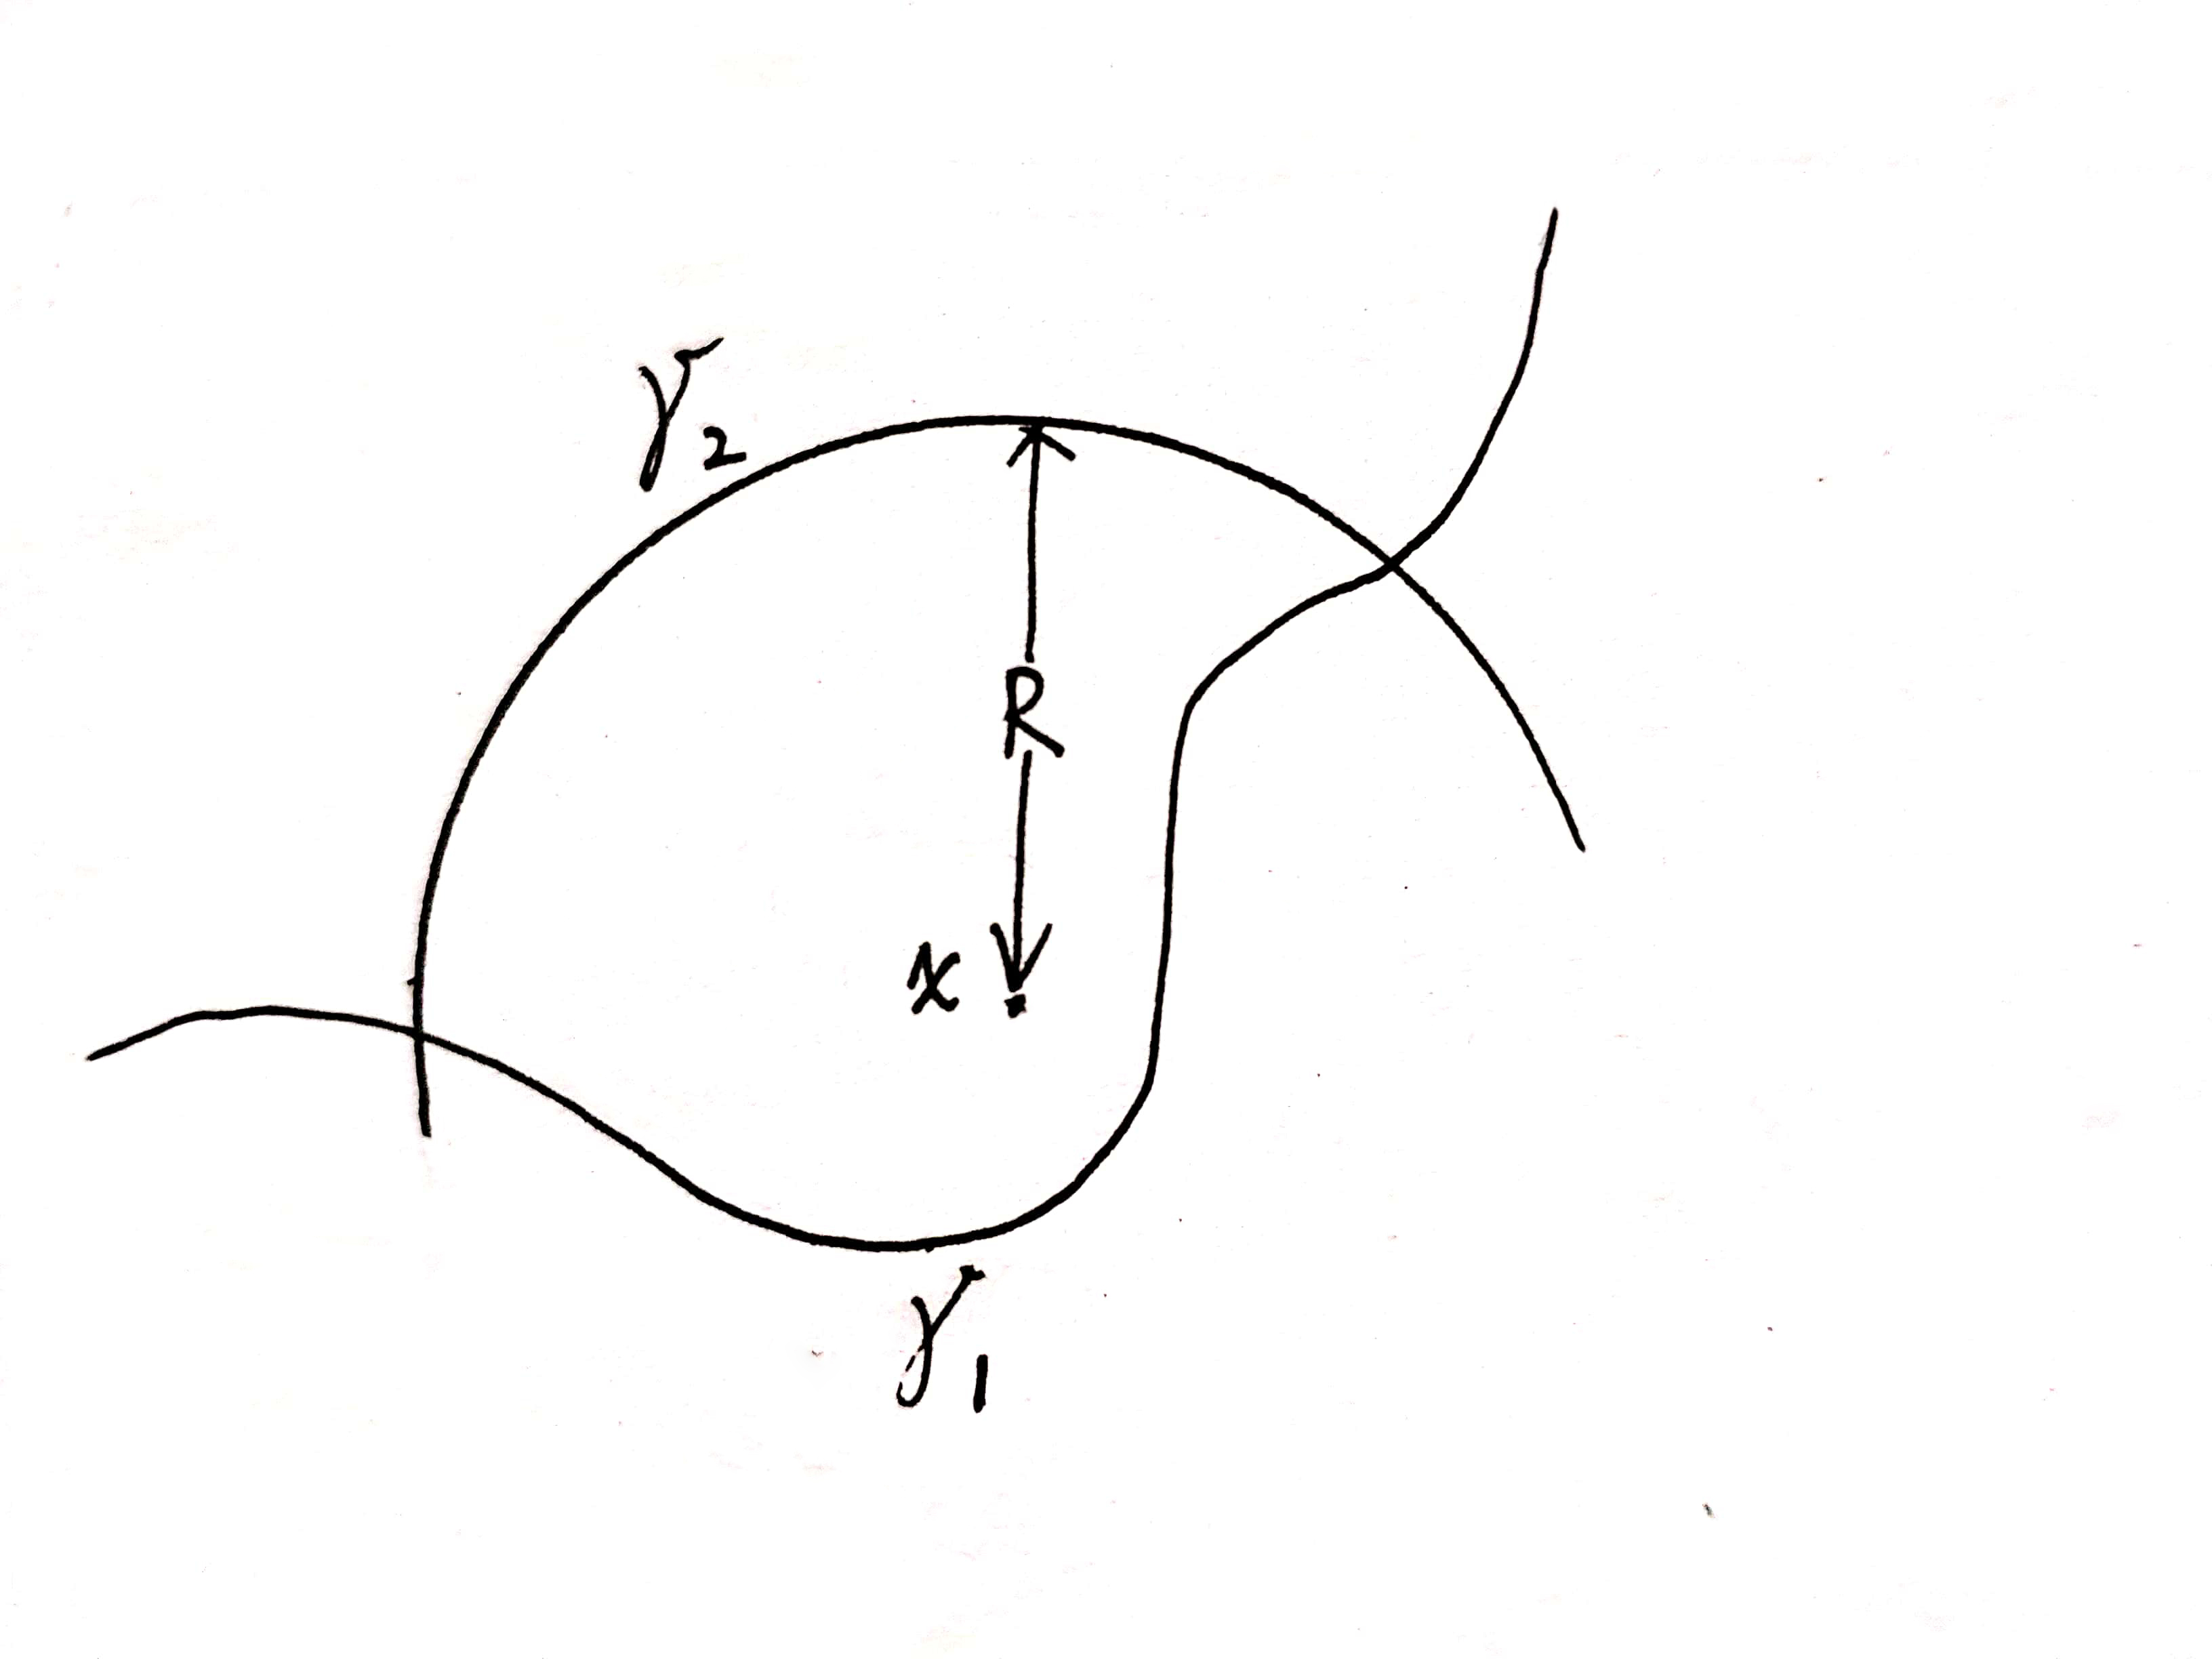
\includegraphics[scale=0.05]{PDE1_4_6.jpg}
        \caption{$\Omega_R$}
        \label{pde1_4_6}
	\end{figure}
	
	于是利用Green公式,对每个固定的$R$,我们可以证明
	\begin{align}
		u(x)&= -\int_{\Omega_R} \Gamma(x-y) \Delta u(y) dy + \int_{\partial \Omega_R} \left(\Gamma(x-y) \frac{\partial u}{\partial \bm{n}_y}(y) -u(y)\frac{\partial \Gamma}{\partial \bm{n}_y}(x,y)   \right) dS_y \notag \\
		&=-\int_{\Omega_R} \Gamma(x-y) \Delta u(y) dy + \int_{\gamma_1} \left(\Gamma(x-y) \frac{\partial u}{\partial \bm{n}_y}(y) -u(y)\frac{\partial \Gamma}{\partial \bm{n}_y}(x,y)   \right) dS_y \notag \\
		&+\int_{\gamma_2} \left(\Gamma(x-y) \frac{\partial u}{\partial \bm{n}_y}(y) -u(y)\frac{\partial \Gamma}{\partial \bm{n}_y}(x,y)   \right) dS_y. \notag
	\end{align}
	显然我们有$$
	\lim_{R \to \infty}	\Omega_R = \Omega ,\qquad \lim_{R \to \infty} \gamma_1 = \partial \Omega, $$
	关键在于证明$$
	\lim_{R \to \infty}\int_{\gamma_2} \left(\Gamma(x-y) \frac{\partial u}{\partial \bm{n}_y}(y) -u(y)\frac{\partial \Gamma}{\partial \bm{n}_y}(x,y)   \right) dS_y =0.	$$
	$n \ge 3$时,
	\begin{align}
		&\quad \lim_{R \to \infty} \left|\int_{\gamma_2} \left(\Gamma(x-y) \frac{\partial u}{\partial \bm{n}_y}(y) -u(y)\frac{\partial \Gamma}{\partial \bm{n}_y}(x,y)   \right) dS_y \right| \notag \\
		&\le \lim_{R \to \infty} C(n) R^{n-1} \left( \left| \Gamma(x-y) \frac{\partial u}{\partial \bm{n}_y}(y) \right|+\left|u(y)\frac{\partial \Gamma}{\partial \bm{n}_y}(x,y)   \right| \right) \notag \\
		&\le \lim_{R \to \infty} C(n) R^{n-1} \left( O\left(\frac{1}{R^{n-2}}\right) \cdot o\left(\frac{1}{R}\right) +o(1) \cdot O\left(\frac{1}{R^{n-1}}\right)   \right) \notag \\
		&= \lim_{R \to \infty} C(n) R^{n-1} \left(  o\left(\frac{1}{R^{n-1}}\right) + o\left(\frac{1}{R^{n-1}}\right) \right) \notag \\
		&= 0 \notag
	\end{align}
	{\color{red}{$n=2$时,上面第一项的估计会难以进行,我们认为需要加强衰减性条件,需要$$
	u(x)=o(1),\qquad |\nabla u(x)|=o\left( \frac{1}{|x|ln|x|} \right), \qquad |x| \to \infty.	$$}}
	在新修订的教材上,添加了这样的条件$\exists a,C >0$,使得$$
	|x|^a u(x)+|x|^{1+a} |Du(x)| + |x|^{2+a} |D^2 u(x)| \le C.	$$
	如此,我们的证明可以进行下去了.其中二阶导数的控制条件应当是为了使得要证的式子第一项积分有意义.

	\subsubsection{$\S_{1.4}$第9题}
	\kaishu{}
	\begin{enumerate}
		\item 求半圆区域上的Dirichlet 问题的Green 函数;
		\item 求$H = \{(x_1, \dots , x_n)|x_{n−1}, x_n > 0\} $上的Dirichlet 问题的Green 函数.
	\end{enumerate}
	
	\subsubsection{$\S_{1.4}$第10题}
	\kaishu{}利用公式(1.54)重新证明单位球上调和函数的Harnack不等式.\\

	\songti{}\uuline{解答}:\\
	
	公式(1.54)指的是$$
	u(x)=-\int_{\partial \Omega} u(y) \frac{\partial G}{\partial \bm{n}_y}dS_y.	$$
	应当指出,书上证明Harnack不等式主要使用的是平均值性质,容易看出公式(1.54)形式上也是一种平均性质.\\
	$\Omega=B_1$,不妨$\Omega^{\prime}$取成半径较小的同心球$B_r$.我们首先指出在单位球面上有$$
	\frac{\partial G}{\partial \bm{n}_y}=- \frac{1-|x|^2}{w_{n-1}|x-y|^n},\qquad \forall n.	$$
	虽然这个等式只要求个导数就能得到,但为了让这份习题解答更受用户的满意,我们决定稍后补上这个等式的证明.现在\begin{align*}
		u(x)&=-\int_{\partial B_1} u(y) \frac{\partial G}{\partial \bm{n}_y}dS_y\\
		&=\int_{\partial B_1} u(y) \frac{1-|x|^2}{w_{n-1}|x-y|^n}dS_y\\
		&\begin{cases}
		\le \frac{1}{(1-r)^n} \frac{1}{w_{n-1}} \int_{\partial B_1} u(y) dS_y\\
		\ge \frac{1-r^2}{(1+r)^n} \frac{1}{w_{n-1}} \int_{\partial B_1} u(y) dS_y
		\end{cases}\\
		&\begin{cases}
		\le \frac{1}{(1-r)^n}  u(0)\\
		\ge \frac{1-r^2}{(1+r)^n}  u(0)
		\end{cases}
	\end{align*}
	接下来的操作和书上的做法是类似的,请读者自行完成.我们接下来将给出单位球面上Green函数的径向导数的公式证明.读者必须注意,虽然维数不同,Green函数的形式略有不同,但它们的径向导数并没有区别,因此我们在这里不对维数$n$进行讨论.\begin{align*}
		\frac{\partial G}{\partial \bm{n}_y}&\xlongequal{\text{单位球面}} \frac{\partial G}{\partial |y|} \\
		&=\frac{\partial G}{\partial y} \cdot \bm{n}_y\\
		&\xlongequal{\text{单位球面}}\frac{\partial G}{\partial y} \cdot y\\
		&=-\frac{1}{w_{n-1}} \left( |x-y|^{-(n-1)}\frac{y-x}{|y-x|}  -\left|\frac{R}{|x|} x -\frac{|x|}{R}y\right|^{-(n-1)} \frac{\frac{|x|}{R}y-\frac{R}{|x|} x}{\left|\frac{|x|}{R}y-\frac{R}{|x|} x\right|}\frac{|x|}{R} \right)\cdot y\\
		&\xlongequal{\text{单位球面}} -\frac{1}{w_{n-1}} \left( |x-y|^{-(n-1)}\frac{y-x}{|y-x|}  -\left|\frac{1}{|x|} x -|x|y\right|^{-(n-1)} \frac{|x|y-\frac{1}{|x|} x}{\left||x|y-\frac{1}{|x|} x\right|}|x| \right)\cdot y \\
		&\xlongequal{|x-y|=\left|\frac{x}{|x|}  -|x|y\right|} -\frac{1}{w_{n-1}|x-y|^n} (y-x-|x|^2 y+x) \cdot y\\
		&\xlongequal{y\cdot y=1}- \frac{1-|x|^2}{w_{n-1}|x-y|^n}.
	\end{align*}
	
	
	
	\subsubsection{$\S_{1.4}$第11题}
	\kaishu{}
	(1) \textbf{Harnack 第一定理}\quad 设函数序列$\{u_k\} \subset  C(\bar{\Omega}) $为$\Omega$上的调和函数列.若$\{u_k\}$ 在$\partial \Omega$ 上一致收敛, 则它在$\Omega$ 上也一致收敛, 并且极限函数$u $也
	是$\Omega $上的调和函数.\\
	
	(2)\textbf{ Harnack 第二定理}\quad 设$\{u_k\}$为$\Omega$上的一个单调不减的调和函数列.若$\{u_k\}$在$\Omega$中的某点P处收敛, 则它内闭一致收敛于$\Omega$ 上的一个调和函数$u $.\\
	
	\songti{}\uuline{解答}:\\
	
	\subsubsection{$\S_{1.4}$第12题}
	\kaishu{}证明Dirichlet 外问题和Dirichlet 问题的等价性. (提示: 利用Kelvin 变换和奇点可去性定理.) 利用该等价性证明有界区域外定义的调和函数若在无穷远
	衰减到0, 则衰减速度至少为$O(\frac{1}{r})$.\\

	\songti{}\uuline{解答}:\\

	\subsubsection{$\S_{1.4}$第13题}
	\kaishu{}证明满足平均值性质的连续函数一定是调和函数.(提示: 利用Poisson 公式和极值原理的证明思想)\\
	
	\songti{}\uuline{解答}:\\
	
	按照提示,设$u$是满足平均值性质的连续函数,由平均值性质可以推出极值原理,故$u$有极值原理.由Poisson公式,记以$u$的边界值为边界的调和函数为$v$,则$u-v$也满足极值原理,但是在边界上取值恒为0,故$u-v\equiv 0$.
	
	另外,也可以先证明$u\in C^{\infty}$,再将证明平均值性质的过程倒推回去即可.事实上,由调和函数的解析性,$u\in C^{\infty}$是显然的.%todo我们给出另外一种利用卷积证明调和函数$u\in C^{\infty}$的办法.
	

\end{document}